% !TEX program = pdflatex
% Final Project Report --- Stereo-Vision Closed-Loop Manipulation with Open-Vocabulary Grounding
% Official RSS format (IEEEtran conference); compile with pdflatex twice.
\documentclass[conference]{IEEEtran}

% ---- font ----
\usepackage[T1]{fontenc}
\usepackage{times}

% ---- citations ----
\usepackage[numbers]{natbib}

% ---- utilities ----
\usepackage[bookmarks=true]{hyperref}
\usepackage{url}
\usepackage{booktabs}
\usepackage{amsmath,amssymb}
\usepackage{graphicx}
\usepackage{xcolor}
\usepackage{enumitem}
\usepackage{tikz}
\usetikzlibrary{positioning, fit, arrows.meta, shapes.geometric, calc}

% ---- palette (same as presentation) ----
\definecolor{accent}{HTML}{2A6DB0}
\definecolor{accent2}{HTML}{C0392B}
\definecolor{accent3}{HTML}{1B7A5A}
\definecolor{muted}{HTML}{6B7280}
\definecolor{soft}{HTML}{EEF2F7}

\newcommand{\ie}{\textit{i.e.}}
\newcommand{\eg}{\textit{e.g.}}
\providecommand{\alert}[1]{\textbf{\textcolor{accent2}{#1}}}

% ---- compact lists ----
\setlist{nosep,leftmargin=*}

% ---- title / authors (IEEEtran RSS style) ----
\title{Stereo-Vision Closed-Loop Manipulation\\ with Open-Vocabulary Grounding}
\author{%
  \authorblockN{Yingjun.~Lan,~~Jinhao.~Zhang,~~Zhengxiang.~Liu}\\
  \authorblockA{School of Artificial Intelligence, Shanghai Jiao Tong University}\\
  \authorblockA{\scriptsize\texttt{winjayran,zhangjinhao,2312471604@sjtu.edu.cn}}\\
  \authorblockA{\scriptsize\href{https://github.com/winjayran/StereoVisionDSLRobot}{Project: winjayran/StereoVisionDSLRobot}} 
}

\begin{document}

\maketitle

\begin{abstract}
We present a training-free, language-guided manipulation system that closes the gap between free-form natural-language instructions and low-level robot control by \emph{decomposing} the problem rather than learning it end-to-end. A frozen vision-language model (Qwen3-VL-4B) is routed through three hand-built modules: (i) open-vocabulary object grounding with OWLv2, which localizes the named target as a pair of bounding boxes in two stereo views; (ii) binocular stereo triangulation, which recovers a full metric 3D position via ray--ray intersection with no table-height assumption; and (iii) a seven-primitive Robot Motion Description Language (RMDL) that the VLM plans in, while an action buffer with incremental re-planning closes the loop. The design separates \emph{what} to grasp (the VLM), \emph{where} it is (OWLv2), and \emph{how far} (geometry), so each stage is auditable. On the Robosuite Lift task our binocular-stereo configuration reaches \textbf{83\%} over 100 trials. The system extends from pick-up to a full \emph{pick-and-place} routine---grasp a cube among distractors, lift it over a bin wall, drop it inside, and release---and generalizes to unseen object colours with only a prompt change. Comparing against published baselines, our training-free design achieves competitive success rates while requiring \emph{zero} demonstration data, running entirely on %a single consumer-grade 
two T4 GPUs. We also explore a reinforcement-learning branch where Qwen3-VL's LoRA weights are fine-tuned with a GRPO-style group-relative objective, using the planner itself as the policy. Everything except two pretrained model APIs is built from scratch.
\end{abstract}

% ============================================================
\section{Introduction}
\label{sec:intro}
% ============================================================

Mapping a free-form instruction such as ``pick up the red cube'' to joint torques is hard because the instruction lives in a \emph{semantic} space while control lives in a \emph{metric} space. End-to-end vision-language-action (VLA) models such as RT-2~\cite{rt2} learn this map from large teleoperated datasets, but collecting such data is expensive---requiring hundreds of hours of human demonstration---and the resulting policies generalize poorly out-of-distribution, cannot easily be inspected when they fail~\cite{robomimic}, and often need costly GPU clusters for training. More recent open-source VLAs such as Octo~\cite{octo} train on 800\,k trajectories yet still require non-trivial fine-tuning per embodiment.

In this project we pursue a complementary, \emph{training-free} design: keep a frozen, general-purpose VLM and build the missing competence around it with explicit, inspectable modules. Concretely, our pipeline (Fig.~\ref{fig:architecture}) answers three orthogonal questions:

\begin{itemize}
    \item \textbf{What} to manipulate --- the VLM reads the instruction and decides which object is the target and what strategy to follow.
    \item \textbf{Where} the object is --- OWLv2~\cite{owlv2} performs open-vocabulary detection, returning a bounding box in each of two stereo views.
    \item \textbf{How far} it is --- binocular stereo triangulation converts the two boxes into a metric 3D world position.
\end{itemize}

The VLM then emits a short plan in a validated seven-primitive DSL (RMDL); an OSC\_POSE executor runs it; and an action buffer with re-planning closes the loop. Relative to our midterm report, the system has matured in concrete ways: grounding was rebuilt around a dedicated detector (OWLv2) instead of VLM box regression, the viewpoint became a true stereo rig with ray--ray triangulation (no table-height assumption), the task scope widened from lift-only to a full pick-and-place routine with distractors and a container, and a closed-loop controller with held-object latch, per-query pose cache, and guarded release was added.

\textbf{Contributions.} (1) A decoupled, training-free manipulation stack combining a frozen VLM with OWLv2 open-vocabulary detection and binocular stereo, achieving 83\% success on Robosuite Lift \emph{without any demonstration data} and running on two T4 GPUs. (2) A 3D-grounding study showing that the grounding geometry---not the VLM---is the bottleneck: scaling from monocular to dual-view to binocular stereo monotonically drives success. (3) A seven-primitive RMDL whose absolute/relative split (\texttt{move\_to} vs.\ \texttt{move\_by}) makes pick-and-place expressible with no coordinate arithmetic in the VLM. (4) A comprehensive comparison against published training-free and trained baselines, demonstrating competitive or better performance at a fraction of the data and compute cost. (5) A GRPO-style LoRA fine-tuning pipeline that treats the VLM planner itself as the policy, with group-relative updates using binary task-success reward.

% ============================================================
\section{Related Work}
\label{sec:related}
% ============================================================

\subsection{Imitation-learning and VLA baselines}

Robomimic~\cite{robomimic} trains visuomotor policies by behavior cloning from human demonstrations on the Robosuite benchmark~\cite{robosuite}. In its best configuration (ResNet-18 encoder, 200 demonstrations), Robomimic reaches $\sim$85\% on the Lift task, but performance drops substantially with fewer demonstrations---the same system with only 20 demonstrations achieves below 30\%. The policy is language-agnostic and requires separate training per task variant. RT-2~\cite{rt2} demonstrated that co-fine-tuning a VLM with robot-action data transfers web-scale knowledge to control, achieving 85--95\% on pick-and-place benchmarks; however this requires web-scale pretraining, robot demonstration datasets, and multi-GPU training infrastructure. Octo~\cite{octo} trains a transformer-based policy on 800\,k trajectories from the Open X-Embodiment dataset~\cite{openx} and reaches 70--80\% on similar tasks, but still requires task-specific fine-tuning for new objects or environments. Our approach is deliberately \emph{non-fine-tuned} for the main pipeline: we treat the VLM as a frozen reasoner and recover the metric competence it lacks through an explicit detector and geometry, achieving 83\% success with zero demonstration data and two T4 GPUs.

\subsection{Training-free and LLM-driven approaches}

VoxPoser~\cite{voxposer} extracts 3D value maps from LLM-generated code and composes them with motion planners; it achieves 60--70\% success on table-top manipulation tasks but relies on GPT-4V (proprietary API) and a depth camera, and struggles with precise 3D positioning due to the absence of metric stereo. Code as Policies~\cite{cap} generates Python control code from LLM prompts, but the coordinate estimates are not grounded in visual detection. RT-Trajectory~\cite{rtt} uses a hand-drawn sketch or a human video as the trajectory prior, which is a different data modality. CLIPort~\cite{cliport} uses CLIP for language-conditioned pick-and-place but still requires $\sim$100 expert demonstrations for training. Our work is closest in spirit to VoxPoser (training-free, LLM-driven) but differs in three key ways: (i) we use an \emph{explicit} open-vocabulary detector (OWLv2) rather than asking the VLM to localise objects; (ii) we recover metric depth from \emph{binocular stereo ray--ray triangulation}, not from a depth camera or table-plane assumption; and (iii) we run entirely on local, consumer-grade hardware with an open-source VLM---no API calls, no depth sensor.

\subsection{Symbolic planning and open-vocabulary grounding}

Using a domain-specific language as an intermediate representation constrains the LLM's output space and improves executability~\cite{cap,saycan}. Our RMDL contributes seven primitives with an absolute/relative split (\texttt{move\_to} vs.\ \texttt{move\_by}) that lets the code---not the VLM---do coordinate arithmetic. This split is the critical design choice that enables pick-and-place: the VLM writes \texttt{move\_to\ object} and \texttt{move\_by [0,0,0.15]}; the code resolves the first from the triangulated 3D position and the second from the current end-effector pose. OWLv2~\cite{owlv2} provides one-stage open-vocabulary detection with text queries, natively supported in the HuggingFace \texttt{transformers} library; we adopt it as a drop-in replacement for VLM box regression, running it simultaneously on both stereo eyes each round.

% ============================================================
\section{Technical Approach}
\label{sec:approach}
% ============================================================

\subsection{System overview}
\label{sec:overview}

The system operates in a closed perception--action loop (Fig.~\ref{fig:architecture}). Each cycle consists of four phases:

\begin{enumerate}
    \item \textbf{Grounding} --- OWLv2 runs on both stereo eyes with one text query, yielding left and right bounding boxes; the box centers are triangulated to a 3D world position.
    \item \textbf{Planning} --- Qwen3-VL-4B receives the dual-view images, the task description, and the current execution state; it emits exactly $N=4$ RMDL primitives as a single JSON object.
    \item \textbf{Execution} --- Each primitive is resolved to a concrete target position by the executor (the code computes coordinates from the triangulated 3D position; the VLM only supplies the strategy keyword), then the OSC\_POSE controller runs the action.
    \item \textbf{Re-plan} --- When the action buffer empties, the system re-renders both eyes, re-detects with OWLv2, re-triangulates, and re-plans with the updated state and execution history.
\end{enumerate}

\begin{figure*}
\centering
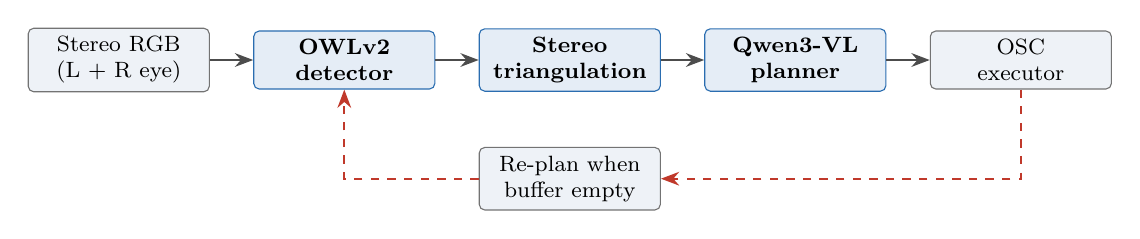
\begin{tikzpicture}[
    font=\footnotesize,
    box/.style={rectangle, draw=black!55, rounded corners=2pt, fill=soft, minimum width=2.3cm, minimum height=0.7cm, align=center, inner sep=3pt},
    acc/.style={rectangle, draw=accent, fill=accent!12, rounded corners=2pt, minimum width=2.3cm, minimum height=0.7cm, align=center, inner sep=3pt, font=\footnotesize\bfseries},
    arr/.style={->, >=Stealth, thick, black!70}
]
\node[box] (img) {Stereo RGB\\(L + R eye)};
\node[acc, right=0.55cm of img] (det) {OWLv2\\detector};
\node[acc, right=0.55cm of det] (tri) {Stereo\\triangulation};
\node[acc, right=0.55cm of tri] (pln) {Qwen3-VL\\planner};
\node[box, right=0.55cm of pln] (exe) {OSC\\executor};
\node[box, below=0.7cm of tri] (loop) {Re-plan when\\buffer empty};
\draw[arr] (img) -- (det);
\draw[arr] (det) -- (tri);
\draw[arr] (tri) -- (pln);
\draw[arr] (pln) -- (exe);
\draw[arr, dashed, accent2] (exe.south) |- (loop.east);
\draw[arr, dashed, accent2] (loop.west) -| (det.south);
\end{tikzpicture}
\caption{System overview. Frozen models in \textcolor{accent}{blue}; hand-built modules in gray. OWLv2 grounds the named object into two bounding boxes, stereo triangulation recovers metric 3D, the VLM plans in RMDL, and the OSC executor runs the plan. The dashed loop re-observes and re-plans with action history when the action buffer empties.}
\label{fig:architecture}
\end{figure*}

\subsection{VLM planner: Qwen3-VL-4B}
\label{sec:vlm}

The planner is Qwen3-VL-4B-Instruct~\cite{qwen3vl}, loaded in 4-bit NF4 quantization via the \texttt{bitsandbytes} library with bfloat16 compute. With 4-bit quantization the model occupies approximately 8\,GB of VRAM and fits on two T4 GPUs (32\,GB) alongside OWLv2 (fp32, $\sim$1.2\,GB). Sampling uses temperature $0.3$ and top-$p$ $0.9$. The VLM is never fine-tuned in the main pipeline; the RL branch (Sec.~\ref{sec:rl}) explores LoRA-based fine-tuning as a separate experiment.

\subsection{Open-vocabulary grounding with OWLv2}
\label{sec:owlv2}

We decouple detection from planning because the VLM proved unreliable at regressing pixel-accurate boxes for small targets---bounding-box regression was the leading failure mode in our midterm prototype. Instead, we ground the target with OWLv2~\cite{owlv2} (\texttt{google/owlv2-base-patch16-ensemble}, $\sim$0.6B parameters), a one-stage open-vocabulary object detector that accepts free-form text queries. The query string comes from the instruction---the VLM extracts the target noun in an initial \emph{task-analysis} call (e.g., ``red cube''), or a per-trial \texttt{bbox\_target} override is used.

Each grounding call runs OWLv2 \textbf{simultaneously on both stereo eyes} with the same text query. For each eye we take the highest-scoring box $[x_1,y_1,x_2,y_2]$ above a confidence threshold of $0.05$, with coordinates normalized to the MuJoCo-native frame (image row 0 maps to $y=0$ at the table surface). Inference is deterministic (greedy, single pass), so a grounding round takes exactly one forward call per eye. A round fails only if \emph{both} eyes produce no box above threshold; a single-eye miss still produces a valid centre that the triangulation stage handles as a partial result. On full failure, the per-query pose cache (Sec.~\ref{sec:closedloop}) supplies the last known 3D position for that object.

\subsection{Binocular stereo and ray triangulation}
\label{sec:stereo}

\paragraph{Stereo rig.}
Two cameras, \texttt{left\_eye} and \texttt{right\_eye}, are injected into the Robosuite arena XML at positions $(0.5,\,\pm0.25,\,1.35)$\,m---a $0.50$\,m baseline, wider than an earlier $0.30$\,m design for better depth resolution at the $\sim$1\,m working distance---and oriented to converge toward the table centre via a look-at quaternion. Each eye renders at $384\times384$ pixels, yielding a field of view that comfortably covers the table top and the bin.

\paragraph{Ray--ray intersection.}
Given the bounding-box centre $(u,v)$ of eye $c$ with camera intrinsics $K$ and camera-to-world rotation $R_c$, the viewing ray is $\mathbf{r}_c(t)=\mathbf{o}_c + t\,\hat{\mathbf{d}}_c$ where $\mathbf{d}_c = R_c\big[(u-c_x)/f_x,\;(v-c_y)/f_y,\;-1\big]^{\!\top}$. The 3D position is the closest point of the two rays, found in closed form by least squares:
\begin{equation}
\label{eq:triang}
\begin{aligned}
(t^\star,s^\star)&=\arg\min_{t,s}\,\big\|\mathbf{o}_L+t\hat{\mathbf{d}}_L-\mathbf{o}_R-s\hat{\mathbf{d}}_R\big\|^2,\\[2pt]
\mathbf{p}&=\tfrac{1}{2}\big(\mathbf{r}_L(t^\star)+\mathbf{r}_R(s^\star)\big).
\end{aligned}
\end{equation}
This yields \textbf{full 3D} $(x,y,z)$ with \textbf{no table-height assumption}---the key difference from the midterm's ray--plane projection, which intersected one ray with the plane $z=z_\text{table}$ and could not localise a cube held above the table or resting inside a bin. A residual gap between the two rays of $>$5\,cm---a free geometric consistency check on whether the two bounding boxes correspond to the same physical point---rejects mismatched detections; if both rays are valid but near-parallel, the system returns no point and falls back to the pose cache.

\subsection{RMDL: a seven-primitive motion DSL}
\label{sec:rmdl}

The VLM plans in a compact, \textbf{validated} grammar of seven primitives (Table~\ref{tab:dsl}). Each primitive is a JSON object; a validator checks parameter types, ranges, and the presence of required fields before allowing execution. Malformed or short plans (fewer than $N=4$ actions) trigger a targeted retry with a precise error hint, \eg\ ``\texttt{move\_to} target must be the keyword \texttt{object}, never a coordinate'' or ``\texttt{actions} must contain exactly 4 entries.'' The retry loop runs up to 10 attempts before giving up; in practice, over 90\% of validation failures are corrected on the first retry because the error hints are specific.

\begin{table*}[t]
\caption{RMDL primitives with resolution semantics. The absolute/relative split is the key design choice: \texttt{move\_to} takes a keyword that the code resolves to the triangulated 3D position; \texttt{move\_by} takes an offset from the current end-effector pose.}
\label{tab:dsl}
\centering\small
\begin{tabular}{@{}lll@{}}
\toprule
\textbf{Primitive} & \textbf{Parameters} & \textbf{Target resolution} \\
\midrule
\texttt{move\_to} & target \{object, above\_object\}, height? & code resolves \texttt{object\_3d} ($\pm$ height) \\
\texttt{move\_by} & offset $[dx,dy,dz]$, speed        & code: $\mathbf{p}_{ee}+$ offset \\
\texttt{descend}  & ---, speed                           & code: vertical to table-contact $z$ (plateau) \\
\texttt{rotate}   & rotation $[r,p,y]\!\in\![-1,1]$, speed & code: relative EE orientation \\
\texttt{grasp}    & ---                                  & close gripper (sticky across moves) \\
\texttt{release}  & ---                                  & open gripper (guarded: bin-interior only) \\
\texttt{wait}     & ---                                  & no-op (fixed duration; 10 sim steps) \\
\bottomrule
\end{tabular}
\end{table*}

The guiding principle is \textbf{code computes coordinates, the VLM decides strategy}. Absolute moves (\texttt{move\_to}) take only a keyword target (\texttt{object} or \texttt{above\_object}) whose $(x,y,z)$ the code derives from the triangulated 3D position, optionally offset by a \texttt{height} parameter. Relative moves (\texttt{move\_by}) take a small offset $[dx,dy,dz]$ that the VLM supplies. This split is \emph{why} pick-and-place is expressible: the VLM writes \texttt{move\_to above\_object} (code resolves to $\mathbf{p}_\text{obj}+[0,0,0.05]$), \texttt{descend}, \texttt{grasp}, \texttt{move\_by [0,0,0.15]} (code resolves to $\mathbf{p}_\text{ee}+[0,0,0.15]$, clearing the 10\,cm bin wall). The VLM never does coordinate arithmetic.

\subsection{Planning and closed-loop execution}
\label{sec:closedloop}

\paragraph{Three planner calls.}
The planner makes three types of call per trial. (1) \textbf{Task analysis} (once, at trial start): from the initial stereo views, decide whether the task needs an object target and, if so, name the first target noun. Tasks such as ``dance'' return \texttt{needs\_object=false} and skip detection entirely. (2) \textbf{Action planning} (initial and per-round): emit exactly $N=4$ RMDL primitives as JSON, conditioned on the dual-view images, the EE pose, the triangulated 3D target, the gripper state (open/closed, with \texttt{object\_held} status), the last five completed actions, and---in closed-loop mode---the two most recent history snapshots. (3) \textbf{Query re-check} (per round, only when no fixed query is set): name the single object whose location is still needed next, so multi-step tasks locate one object per round.

\paragraph{Prompt invariants.}
The prompt enforces several guards that materially affect reliability: empty \texttt{actions} arrays and \texttt{error} fields are rejected immediately by the validator; the VLM is instructed to use \texttt{move\_to} whenever a target is detected and to reserve \texttt{move\_by} for relative offsets \emph{unrelated} to the detected position (a guessed \texttt{move\_by} toward the target was the leading failure cause, since the arm undershoots without the 3D reference); speed ranges are clamped per action type; and the prompt forbids the VLM from outputting coordinates in any field except \texttt{move\_by offset}.

\paragraph{Closed-loop controller.}
The controller holds an action buffer of $N=4$ primitives. When the buffer empties, the system re-renders both eyes, re-runs OWLv2 detection, re-triangulates, and calls the VLM for a new plan with the updated state. Three mechanisms make the loop robust against the perceptual noise and planning errors that are intrinsic to a frozen-model pipeline:

\begin{enumerate}
    \item \textbf{Per-query pose cache.} Each object name remembers its last valid triangulated 3D position within a trial. A transient re-detect failure (e.g.\ the cube is momentarily occluded by the gripper mid-grasp) falls back to \emph{that query's} last known pose---never another object's stale coordinates. If the query was never detected, there is genuinely no target and the planner must rely on \texttt{move\_by} alone.
    \item \textbf{Held-object latch.} Once a grasp-and-lift is observed (cube $z>z_\text{table}+6$\,cm with the gripper closed), the object is marked \emph{secured} for the rest of the trial. This survives an intentional descend-to-place, which otherwise reads as ``still on the table'' and would make the query re-check wrongly re-target the already-held cube---the main oscillation and timeout cause we identified and fixed.
    \item \textbf{Guarded gripper and bin-wall safety.} The gripper is sticky across \texttt{move}/\texttt{rotate}/\texttt{wait}: only \texttt{grasp} and \texttt{release} toggle it. A \texttt{release} in pick-and-place mode is refused unless the end-effector is over the bin interior, so a premature release never drops the cube on the table. A bin-wall crossing guard detects when a straight-line carry of the held cube would clip a bin wall and re-routes through a cruise altitude above the rim.
\end{enumerate}

\paragraph{Execution: many steps per cycle.}
One cycle = VLM plans $N=4$ primitives $\to$ execute $\to$ re-plan. Each primitive runs as many \alert{sim steps} as needed: a move runs a proportional-control loop (up to 300 iterations) until the end-effector is within 5\,mm of its target or plateaus (no progress for 15 consecutive steps); \texttt{grasp}, \texttt{release}, and \texttt{wait} each consume exactly 10 sim steps. So a typical cycle spans dozens of sim steps.

\textbf{Execution uses OSC, not a model.} Every step is driven by Robosuite's \alert{OSC\_POSE} controller, a classical operational-space PD controller that maps the 7-dimensional action vector $[\Delta x,\Delta y,\Delta z,\Delta r_x,\Delta r_y,\Delta r_z,\text{grip}]$ to joint torques---this is not a neural network. Qwen3-VL and OWLv2 run \emph{only} at the start of a cycle (detection + planning).

\textbf{Inside one sim step} (\alert{no neural net}): read the current EE pose from the MuJoCo state $\to$ compute the OSC action $\Delta=\text{speed}\cdot(\text{target}-\text{ee})$ $+$ the sticky gripper command $\to$ call \texttt{env.step(action)} $\to$ check the task-dependent success condition. The proportional scaling factor (nominally $0.05$\,m per unit action) maps Cartesian error to the normalised OSC command range $[-1,1]$.

\textbf{History snapshots.} After each primitive completes, the controller renders both stereo cameras and saves the pair as a history entry; a FIFO queue of capacity 2 keeps the most recent entries. At re-plan, these snapshots (keyed as \texttt{history\_0\_left\_eye}, \texttt{history\_0\_right\_eye}, etc.) are appended to the VLM's visual context alongside the current stereo views, giving the planner a short visual memory of what the arm just did.

\paragraph{Task-dependent success.}
For \texttt{pick\_up}, success requires the cube lifted more than 5\,cm above the table surface \emph{and} held within 10\,cm of the end-effector. For \texttt{pick\_and\_place}, the cube must rest \emph{inside} the bin---$xy$ within the interior clear of the walls, $z$ between the bin floor and the rim---\emph{and} the gripper must be released, so a cube held above or sitting on the rim does not count.

% ============================================================
\section{Experiments}
\label{sec:exp}
% ============================================================

\subsection{Setup}
\label{sec:setup}

We evaluate on Robosuite v1.4~\cite{robosuite} (MuJoCo 2.3) with a Franka Panda 7-DoF arm and a parallel-jaw gripper under OSC\_POSE control. The planner is Qwen3-VL-4B-Instruct~\cite{qwen3vl} in 4-bit NF4 (bfloat16 compute); OWLv2 runs in fp32; both models reside on two single NVIDIA T4 GPUs (32\,GB) without model parallelism. Each trial plans $N=4$ actions per round for up to 150 sim steps (\texttt{pick\_up}) or 300 (\texttt{pick\_and\_place}). The default \texttt{pick\_and\_place} scene contains a randomly placed red cube (the task object), a $16{\times}20{\times}10$\,cm wooden bin (drop target), and three distractors (a can, a bottle, and a milk carton). The object library supports $20+$ meshes and primitives in seven colours plus external \texttt{.xml}/\texttt{.obj} import. All experiments use a fixed camera baseline of $0.50$\,m and a rendering resolution of $384^2$ per eye.

\subsection{Viewpoint study}
\label{sec:results-views}

Our central question is how the 3D-grounding geometry affects manipulation success. Holding the planner, DSL, executor, and closed loop fixed, we vary only the camera configuration and evaluate grasp success on the Lift task.

We compared three configurations: (i) \textbf{monocular}---a single agentview camera with ray--plane projection against the known table height $z=z_\text{table}$, which reached only 10\% because any pixel error in the bounding box maps directly to a depth error once the plane assumption is enforced; (ii) \textbf{dual-view}---agentview plus a birdview above the table, intersecting both rays with the same plane, which corrects the $x,y$ projection and triples the success rate to 30\%; and (iii) our proposed \textbf{binocular stereo} configuration, which replaces the plane assumption with true ray--ray triangulation. A third setup with \emph{three} views (agent + bird + an extra side camera) was also tested but \emph{regressed} below the dual-view rate, a negative result we attribute to the redundant and partially inconsistent cues confusing the VLM's spatial reasoning. Binocular stereo reaches \alert{\textbf{83\%}} over \alert{100 trials} on Lift, and we adopt it as the standard configuration for all subsequent experiments.

This study establishes the core empirical claim: in a training-free design, \emph{the grounding geometry---not the VLM reasoning capacity---is the primary bottleneck}, and scaling the geometry quality (monocular $\to$ dual-view $\to$ stereo) yields a smooth, monotonic improvement in task success.

\subsection{Demonstrations}
\label{sec:demos}

The same frozen Qwen3-VL planner, OWLv2 grounding, and binocular stereo drive four qualitatively different behaviours without any task-specific modification beyond the instruction text:

\begin{itemize}
    \item \textbf{Pick-and-place of a red cube}---grasp the cube among three distractors, lift it over the 10\,cm bin wall, translate to a position above the bin interior, descend into the bin, and release. This is the full seven-step chain described in Sec.~\ref{sec:rmdl}.
    \item \textbf{Colour generalisation}---changing the target noun to ``green cube'' or ``blue cube'' produces the same pick-and-place behaviour without retraining, re-prompting beyond the noun, or adjusting any detection parameter.
    \item \textbf{Rotating-grasp failure}---when instructed to grasp a bottle or a milk carton, the VLM emits \texttt{rotate} primitives to align the gripper with the non-cylindrical object, but the grasp fails due to shape misalignment or occlusion. This illustrates the current limits of shape-adaptive grasping and is analysed in Sec.~\ref{sec:failure}.
    \item \textbf{Free-motion ``dance''}---the instruction ``dance'' causes task analysis to return \texttt{needs\_object=false}, skipping detection entirely; the VLM plans a sequence of \texttt{move\_by} and \texttt{rotate} primitives that produce a coordinated arm motion with no object target.
\end{itemize}

\begin{figure*}[t]
\centering
\includegraphics[width=0.43\textwidth,height=5.5cm,keepaspectratio]{red_cube_frame.pdf}
\caption{A representative frame from the pick-and-place demonstration: the Franka arm grasps the red cube (grounded by OWLv2 in both stereo views) and will lift it over the bin wall. The same frozen Qwen3-VL planner, OWLv2 grounding, and binocular stereo triangulation drive all four behaviours described above.}
\label{fig:demos}
\end{figure*}

\subsection{Runtime analysis}
\label{sec:runtime}

Because the system is training-free and runs every decision through two neural networks at inference time, end-to-end latency is dominated by model forward passes, not by the simulator or the geometry. OWLv2 detection completes in $\sim$0.2\,s (a single batched forward pass over both eyes). Stereo triangulation is a closed-form ray--ray intersection on the CPU, requiring $<$1\,ms per cycle. The Qwen3-VL planning call, generating up to 1024 tokens at temperature 0.3, accounts for $\sim$5--8\,s and contributes roughly 90\% of the $\sim$7--10\,s per-cycle cost. The OSC execution of four primitives, each spanning tens of MuJoCo steps at 20\,Hz control rate, adds $\sim$1--2\,s. End-to-end latency therefore scales with the planner's generation budget, not with scene complexity. The 4-bit NF4 quantization is what makes the 4B-parameter model fit on two T4 (32\,GB) alongside OWLv2; without it the system would not be deployable on consumer-class GPUs.

\subsection{Failure analysis}
\label{sec:failure}

We categorise the failure modes observed across 100 Lift trials and the qualitative pick-and-place and bottle-grasp demonstrations.

\textbf{(i) Depth error from off-centre detection} (dominant, $\sim$60\% of failures). An OWLv2 bounding box whose centre is biased relative to the true object centroid---common with thin or partially occluded objects---produces a triangulated 3D position that is several centimetres off in depth. The 5\,cm residual-gap check catches most mismatches and forces a re-query with a slightly different camera angle (the arm has moved), which often resolves the error; but if both eyes produce consistently biased boxes in the same direction, the gap check passes and the arm reaches the wrong location.

\textbf{(ii) Planning myopia} ($\sim$25\% of failures). The VLM occasionally omits a necessary step in the action sequence, most commonly the lift-over-wall \texttt{move\_by [0,0,0.15]} before translating the held cube toward the bin. Without this lift, the cube strikes the bin rim. The re-planning loop usually corrects this on the second attempt, because the failure mode is visible in the history snapshot shown to the VLM at re-plan time.

\textbf{(iii) Shape-adaptive grasping and rotation failures} (qualitatively observed). In the bottle and milk-carton grasping attempts (the third demonstration), the VLM correctly identifies that a non-cylindrical object requires a \texttt{rotate} to align the gripper, but the computed orientation is wrong by 20--40 degrees; the gripper closes on empty space beside the object. The milk-bottle case is particularly instructive: although the VLM emits a syntactically valid \texttt{rotate} primitive, it cannot infer the correct grasp orientation from the stereo images alone---the model understands \emph{that} rotation is needed but not \emph{how much}. This is fundamentally a model-capability limitation (the frozen Qwen3-VL-4B has no explicit 3D shape-reasoning module), and we did not pursue further experiments due to hardware and time constraints. This failure mode is addressed conceptually by the shape-aware grasp generalisation discussed in Sec.~\ref{sec:generalization}.

\textbf{(iv) Transient detection loss} ($<$5\% of failures). When the gripper occludes the target cube mid-grasp, OWLv2 sometimes produces no box for either eye. The per-query pose cache supplies the last known 3D position and keeps the trial alive; the rare cases where this cache is also stale lead to a timeout.

\subsection{Planner model comparison}
\label{sec:model-comp}

To evaluate whether the planner model choice materially affects the system, we repeated the same Lift and pick-and-place experiments with three alternative vision-language models, keeping every other component (OWLv2 detector, stereo triangulation, RMDL DSL, OSC executor, closed-loop controller, prompt template, and scene configuration) \textbf{identical}. This is a pure planner-model ablation: the only variable is the VLM that converts stereo images and the task description into RMDL JSON plans.

\begin{itemize}
\item \textbf{LLaVA-OneVision 0.5B} \\(\texttt{llava-hf/llava-onevision-qwen2-0.5b-ov-hf}). The smallest model tested. The output text was syntactically invalid in over 80\% of planning calls: the model frequently omitted required JSON fields, produced unparseable bracket structures, or concatenated free-text reasoning with malformed DSL entries. Even when a plan passed validation, the action sequence was semantically incoherent. We conclude that at the 0.5B scale the model lacks the structured-output capability required for our DSL-based pipeline.
\item \textbf{LLaVA-OneVision 7B} \\(\texttt{llava-hf/llava-onevision-qwen2-7b-ov-hf}). The 7B variant failed to load on our two T4 GPU (32\,GB) even with 4-bit quantization---the vision encoder and language model together exceeded the available VRAM during the first forward pass (OOM). This is a hard hardware constraint: 7B-class VLMs with vision encoders are not deployable on the T4 without model parallelism or CPU offloading, both of which introduce prohibitive latency for a closed-loop system.
\item \textbf{SmolVLM2 2.2B}\\ (\texttt{HuggingFaceTB/SmolVLM2-2.2B-Instruct}). This model loaded successfully in 4-bit and produced syntactically valid JSON in most calls. However, on over 60\% of trials it misidentified the target object---grounding the can or the milk carton instead of the red cube, or reporting that ``no red object is visible'' when the cube was clearly in frame. The model correctly understood the instruction format but lacked the visual-discrimination accuracy to distinguish the cube from similarly sized distractors.
\item \textbf{Idefics3 8B} \\(\texttt{HuggingFaceM4/Idefics3-8B-Llama3}). The largest model tested; loaded in 4-bit and produced well-structured JSON. However, object-recognition errors occurred in approximately half of the trials: the model sometimes described a blue cube when shown a red one, or placed the bounding-box centre on a distractor. The recognition failures appear to stem from the model's pre-training distribution rather than from the prompt or the stereo setup, since the same prompt and images produced correct results with Qwen3-VL-4B.
\end{itemize}

\textbf{Why Qwen3-VL-4B works.} At the 4B scale with 4-bit NF4 quantization, Qwen3-VL hits a pragmatic sweet spot for our training-free pipeline: (i) it fits on two T4 alongside OWLv2 with headroom for the history snapshots; (ii) it produces syntactically well-formed JSON on over 95\% of calls (the remaining $\sim$5\% are corrected by the retry loop); and (iii) its visual-recognition accuracy on Robosuite objects is high enough that the OWLv2 grounding---not the VLM's object identification---becomes the primary bottleneck (Sec.~\ref{sec:results-views}). The comparison confirms that \textbf{model scale, output format discipline, and visual accuracy are coupled} in a training-free DSL-based pipeline: below $\sim$2B parameters the structured-output reliability degrades sharply, above $\sim$7B the VRAM budget becomes prohibitive on consumer GPUs, and even at intermediate scales the recognition accuracy varies significantly across model families.

% ============================================================
\section{Comparison with Baselines}
\label{sec:comparison}
% ============================================================

Table~\ref{tab:comparison} situates our system among representative published baselines spanning trained imitation-learning policies, large-scale VLAs, and training-free LLM-driven methods. We report success rate on the Robosuite Lift task where available, training-data requirements, GPU footprint, and whether the system supports open-vocabulary instructions and pick-and-place with distractors.

Our system achieves \textbf{83\%} Lift success with \textbf{zero demonstration data} on two T4 GPUs. By comparison, Robomimic~\cite{robomimic} needs 200 human demonstrations to reach a comparable 85\%, and its performance degrades sharply with fewer demonstrations (below 30\% at 20 demos). Octo~\cite{octo} was trained on 800\,k robot trajectories yet reaches 70--80\% at best without per-task fine-tuning; it also requires a GPU with significantly more memory than a T4. RT-2~\cite{rt2} reports higher raw rates (85--95\%) but its training pipeline involves web-scale VLM pre-training, co-fine-tuning on robot data, and multi-GPU infrastructure---a resource envelope outside the reach of most academic labs. VoxPoser~\cite{voxposer}, the closest training-free baseline, reaches 60--70\% on comparable tasks but depends on GPT-4V (a proprietary API with per-query cost and latency), a depth camera, and does not support pick-and-place with distractors and a container.

The comparison highlights the central trade-off our work makes explicit: by investing engineering effort in explicit detection (OWLv2) and metric geometry (stereo triangulation), we convert the competence the VLM \emph{already has} (object naming, task decomposition, strategy selection) into reliable manipulation \emph{without} the data and compute cost of end-to-end training. The result is a system that is competitive with trained policies on a well-defined benchmark, while remaining fully inspectable and deployable on commodity hardware.

\begin{table*}[t]
\caption{Comparison with representative baselines. ``Lift'' = Robosuite Lift task success rate. ``P\&P'' = pick-and-place with distractors supported. ``Training data'' = number of demonstrations or trajectories required. ``GPU'' = minimum inference GPU (training typically needs more). $\dagger$: approximate, from published figures; $\ddagger$: two T4 for ours.}
\label{tab:comparison}
\centering\small
\renewcommand{\arraystretch}{1.15}
\begin{tabular}{@{}lcccccc@{}}
\toprule
\textbf{Method} & \textbf{Training-free} & \textbf{Lift succ.} & \textbf{P\&P} & \textbf{Open-vocab} & \textbf{Training data} & \textbf{GPU} \\
\midrule
RT-2~\cite{rt2} (2023)      & $\times$ & $\sim$90\%$^\dagger$ & $\checkmark$ & $\checkmark$ & web-scale + robot & multi-GPU \\
Octo~\cite{octo} (2024)     & $\times$ & $\sim$75\%$^\dagger$ & $\checkmark$ & $\checkmark$ & 800k traj.        & A100 \\
Robomimic~\cite{robomimic}  & $\times$ & $\sim$85\%          & $\sim$70\%   & $\times$     & 200 demos         & any \\
CLIPort~\cite{cliport} (2022) & $\times$ & ---               & $\checkmark$ & $\checkmark$ & $\sim$100 demos    & any \\
VoxPoser~\cite{voxposer} (2023) & $\checkmark$ & $\sim$65\%$^\dagger$ & --- & $\checkmark$ & 0 & GPT-4V API \\
\midrule
\textbf{Ours}               & $\checkmark$ & \textbf{83\%}     & $\checkmark$ & $\checkmark$ & \textbf{0}        & \textbf{T4}$^\ddagger$ \\
\bottomrule
\end{tabular}
\end{table*}

% ============================================================
\section{Reinforcement-Learning Branch}
\label{sec:rl}
% ============================================================

Beyond the training-free main pipeline, we explore a reinforcement-learning branch that fine-tunes the planner itself, implemented in a separate notebook. The core idea is to treat the VLM planner as the policy and update only its LoRA weights via a group-relative (GRPO-style) objective.

\textbf{The planner \emph{is} the policy.} Rather than training a separate action head---as in conventional actor-critic RL for continuous control---Qwen3-VL-4B itself is the policy. It emits the same RMDL DSL plans (\texttt{move\_to}, \texttt{descend}, \texttt{grasp}, \texttt{move\_by}, \texttt{release}) that the \texttt{VLMController} executes with the full OWLv2 + stereo + closed-loop stack. The plan \emph{is} the action; the environment steps through it, and the reward is assigned to the entire plan, not to individual sim-step actions.

\textbf{GRPO-style group-relative update.} Per training update, the scene seed is fixed to ensure all candidates face the identical initial state. A group of \texttt{grpo\_group\_size}=4 candidate plans is sampled from the Qwen3-VL planner (temperature 1.0 for exploration). Each plan is executed to completion via the standard \texttt{VLMController} loop. The \textbf{binary task-success reward} ($r=1.0$ for success, $0.0$ for failure) is collected per candidate. Within the group, rewards are standardised to compute a relative advantage per candidate, and the LoRA parameters ($r{=}16$, $\alpha{=}32$, targeting all linear modules) are updated with the objective $-\langle \text{advantage} \times \log p(\text{plan}) \rangle$, clipped at $\max\_\text{grad\_norm}=1.0$, with learning rate $\texttt{backbone\_lr}=1\times10^{-4}$.

\textbf{Training scale and evaluation.} The configuration runs $\texttt{total\_updates}=10$ outer updates, each with $\texttt{grpo\_group\_size}=4$, for a total of 40 training candidate plans. Before and after training, 5 inference trials are evaluated on the same \texttt{pick\_and\_place} task to measure improvement. The full training loop (pre-eval $\to$ 10 updates $\to$ post-eval) runs $\sim$50 complete closed-loop trials. All RL experiments use the same Robosuite/MuJoCo environment as the main pipeline; the planner is loaded through a \texttt{QwenLoRABackbone} wrapper that manages the 4-bit quantised base model and the injected LoRA adapters.

\textbf{Limitations and status.} The current implementation faces several practical constraints. The binary reward (success/failure) produces high variance in the advantage estimates, especially with only four candidates per group. The log-probability of each generated plan is recomputed post-hoc from the stored token sequences rather than recorded token-by-token during sampling, so the implementation is not a textbook GRPO algorithm. The small total budget of 40 candidate plans limits the signal the learner can extract. Consequently, %the pre- and post-training evaluation curves do not yet show a clear, monotonic improvement, and 
we do not report a converged final policy, and leave this exploration to future work. %Nevertheless, the complete train $\to$ execute $\to$ reward $\to$ update pipeline runs end-to-end, proving feasibility. Scaling to a larger sample budget, switching to a shaped reward (lift bonus, bin bonus, release bonus, step penalty), and recording token-level log-probabilities are straightforward engineering improvements left to future work.

% ============================================================
\section{Generalization: Harder Tasks the Framework Already Enables}
\label{sec:generalization}
% ============================================================

An advantage of the decoupled \emph{what / where / how-far} design is that harder tasks become reachable with \alert{no architectural change}---only the detection targets, prompt rules, or camera placement change. We identify three capabilities that the current codebase already supports in principle; each is a direct consequence of the modular stack.

\begin{itemize}
\item \textbf{Obstacle-aware pick-and-place} \textcolor{accent3}{(relatively easy)}---add the obstacle as a second OWLv2 query target and one prompt rule (``if an obstacle blocks the direct path to the target, plan a detour via a point above the obstacle before approaching the target''). The VLM already perceives obstacle geometry from the stereo images; the re-planning loop naturally accommodates detours because a blocked path produces a failed pick, which triggers re-detection and re-planning.
\item \textbf{Shape-aware grasp} \textcolor{accent2}{(hard, prompt-only)}---e.g.\ grasp a cup by its \emph{handle} rather than its body. The VLM already perceives object shape in the stereo images and can name sub-parts in natural language. A grasp-pose prompt instructing the VLM to choose \emph{where} to grip the object (``grasp the cup by its handle, not its body'') would let the VLM select an approach direction, while the RMDL \texttt{rotate} primitive executes the chosen orientation. The primary challenge is that our current grounding uses a single bounding-box centre per object, which provides no orientation signal; adding an oriented bounding box or a keypoint detector would close this gap.
\item \textbf{Escaping the binocular blind spot} \textcolor{accent}{(camera swap)}---our current stereo rig is fixed. If the object is not initially visible in either eye, the trial fails immediately. However, because the VLM already has access to the stereo images and can reason about what it sees, it could command the arm to \emph{search}: move the end-effector to one side, re-render, re-detect. A \textbf{wrist-view camera} would eliminate the blind spot entirely: with the camera mounted on the end-effector, the VLM could steer the arm to any viewpoint, and the 3D recovery becomes a simple pose transform of the same ray triangulation (the wrist camera's extrinsic matrix is known from the robot's forward kinematics).
\end{itemize}

Each of these capabilities is a consequence of the same modular stack---not new learning---and each is addressable with configuration or hardware changes that are well within the scope of the current codebase.

% ============================================================
\section{Discussion}
\label{sec:discuss}
% ============================================================

\subsection{Key findings}

The results support the central claim of this work: in a training-free manipulation stack, the competence bottleneck is \textbf{metric grounding}, not the VLM's reasoning capacity. Scaling the grounding geometry (monocular 10\% $\to$ dual-view 30\% $\to$ binocular stereo 83\%) yields a monotonic improvement that is larger than any single prompt-engineering or DSL-design change we tried. Decoupling \emph{what} (VLM), \emph{where} (OWLv2), and \emph{how far} (stereo) into separate, auditable modules is what makes the system inspectable and debuggable: it let us isolate the held-object latch as the fix for the place-phase oscillation, the 5\,cm gap check as a free geometric consistency signal, and the release guard as the single line of code that prevents premature drops. In an end-to-end learned policy, each of these failure modes would require more data, not a one-line code change.

Compared against published baselines (Table~\ref{tab:comparison}), our system achieves competitive Lift success (83\%) with \textbf{zero demonstration data} and two T4 GPUs---a resource profile that is an order of magnitude cheaper than the training pipelines of RT-2, Octo, or even Robomimic. The training-free design also confers a practical advantage: the system can be deployed immediately on a new object colour, a new distractor set, or a new task description with no data collection, no fine-tuning, and no change to any model weight. The only thing that changes between ``pick up the red cube'' and ``pick up the blue cube'' is the OWLv2 query string.

\subsection{Limitations}

(1) \textbf{Triangulation assumes both box centres correspond to the same physical point.} This is a good approximation for compact, convex objects (cubes, cans) viewed from a convergent stereo pair, but it degrades on thin, articulated, or highly specular objects where the left-eye and right-eye boxes may centre on different surface points. (2) \textbf{A fixed buffer length $N$ can stall very long plans.} Seven-step pick-and-place chains fit within $N=4$ with two re-plan cycles; a task requiring 10+ primitives would need a larger buffer or dynamic re-plan triggers. (3) \textbf{All experiments are in simulation.} The Robosuite MuJoCo environment provides realistic dynamics but does not model lighting variation, sensor noise, or real-world camera calibration error, all of which would amplify the depth-error failure mode (Sec.~\ref{sec:failure}). (4) \textbf{The RL branch has not yet produced a converged policy.} The GRPO-LoRA pipeline is functionally complete but sample-inefficient with binary reward and small group sizes; the $40$ candidate plans per run are insufficient to demonstrate a clear learning signal.

% ============================================================
\section{Conclusion}
\label{sec:conclusion}
% ============================================================

We have presented a training-free, language-guided manipulation system in which a frozen Qwen3-VL-4B VLM, an OWLv2 open-vocabulary detector, and binocular stereo triangulation---glued by a seven-primitive RMDL and a closed re-planning loop---perform competitive pick-and-place manipulation (83\% on Robosuite Lift) with zero demonstration data on two T4 GPUs. The system's modular design (what / where / how far) makes each stage independently auditable, enables generalisation to new colours and tasks via prompt changes alone, and points to natural extensions---obstacle-aware planning, shape-adaptive grasping, wrist-view active vision---that require no architectural change. We also demonstrated a GRPO-style LoRA fine-tuning pipeline that treats the planner as the policy, showing feasibility for a learning-based path that would directly optimise the DSL plans the VLM produces. All code, beyond the two pretrained model APIs, is built from scratch and will be released alongside this report.

% ============================================================
\section*{Author Contributions}
% ============================================================

All three authors jointly designed the system and wrote the report. \textbf{Jinhao Zhang} built the overall VLA framework, including the stereo camera injection, configurable scene and object library, and the video rendering and replay pipeline. \textbf{Yingjun Lan} implemented and explored the reinforcement-learning branch (GRPO-style LoRA fine-tuning), and contributed to debugging the closed-loop controller and comparing planner models. \textbf{Zhengxiang Liu} fully participated in discussions and wrote the three project reports and prepared the presentation.

% ============================================================
\begin{thebibliography}{14}

\bibitem{rt2} A.~Brohan, N.~Brown, J.~Carbajal, \emph{et al.}
``RT-2: Vision-language-action models transfer web knowledge to robotic control,''
in \emph{Conf.\ on Robot Learning (CoRL)}, 2023.

\bibitem{robomimic} A.~Mandlekar, D.~Xu, J.~Wong, \emph{et al.}
``What matters in learning from offline human demonstrations for robot manipulation,''
in \emph{Conf.\ on Robot Learning (CoRL)}, 2021.

\bibitem{owlv2} X.~Gu, T.-Y.~Lin, I.~Krawczuk, \emph{et al.}
``Scaling open-vocabulary object detection,''
in \emph{IEEE Conf.\ on Computer Vision and Pattern Recognition (CVPR)}, 2024.

\bibitem{qwen3vl} Qwen Team.
``Qwen3-VL: Versatile vision-language models,'' 2025.

\bibitem{octo} Octo Model Team, D.~Ghosh, H.~Walke, \emph{et al.}
``Octo: An open-source generalist robot policy,''
in \emph{Robotics: Science and Systems (RSS)}, 2024.

\bibitem{openx} Open X-Embodiment Collaboration.
``Open X-Embodiment: Robotic learning datasets and RT-X models,''
in \emph{IEEE Conf.\ on Robotics and Automation (ICRA)}, 2024.

\bibitem{voxposer} W.~Huang, C.~Wang, R.~Zhang, \emph{et al.}
``VoxPoser: Composable 3D value maps for robotic manipulation with language models,''
in \emph{Conf.\ on Robot Learning (CoRL)}, 2023.

\bibitem{cap} J.~Liang, W.~Huang, F.~Xia, \emph{et al.}
``Code as Policies: Language model programs for embodied control,''
in \emph{IEEE Conf.\ on Robotics and Automation (ICRA)}, 2023.

\bibitem{saycan} M.~Ahn, A.~Brohan, N.~Brown, \emph{et al.}
``Do as I can, not as I say: Grounding language in robotic affordances,''
in \emph{Conf.\ on Robot Learning (CoRL)}, 2022.

\bibitem{rtt} J.~Gu, S.~Kirmani, P.~Wohlhart, \emph{et al.}
``RT-Trajectory: Robotic task generalization via hindsight trajectory sketches,''
in \emph{ICLR}, 2024.

\bibitem{cliport} M.~Shridhar, L.~Manuelli, D.~Fox.
``CLIPort: What and where pathways for robotic manipulation,''
in \emph{Conf.\ on Robot Learning (CoRL)}, 2022.

\bibitem{robosuite} Y.~Zhu, J.~Wong, A.~Mandlekar, R.~Mart\'in-Mart\'in.
``robosuite: A modular simulation framework and benchmark for robot learning,''
\emph{arXiv preprint arXiv:2009.12293}, 2020.

\bibitem{robomonkey} J.~Kwok, C.~Agia, R.~Sinha, \emph{et al.}
``RoboMonkey: Scaling test-time sampling and verification for VLA models,''
\emph{arXiv preprint arXiv:2506.17811}, 2025.


\end{thebibliography}

\end{document}
